\section{Provas dos teoremas}
 
%%%%%%%%%%%%%%%%%%%%%%%%%%%%%%%%%%%%%%%%%%%%%%%%%%%%%%%%%%%%%%%%%%%%%%%%%%%%%%%%%%%%%%%
%%%%%%%%%%%%%%%%%%%%%%%%%%%%%%%%%%%%%%%%%%%%%%%%%%%%%%%%%%%%%%%%%%%%%%%%%%%%%%%%%%%%%%%
\begin{myproofT}[Relativa ao Teorema \ref{theo:minAxbCAxb}:]\label{proof:theo:minAxbCAxb}
Dados,
os vetores coluna $\VECTOR{x}\in \mathbb{R}^N$ e $\VECTOR{b}\in \mathbb{R}^M$,  
uma matriz $\MATRIX{A} \in \mathbb{R}^{M\times N}$, 
uma matriz diagonal $\MATRIX{C} \in \mathbb{R}^{M\times M}_+$, e 
definida a Eq. (\ref{eq:proof:minAxbCAxb0}),
\begin{equation}\label{eq:proof:minAxbCAxb0}
e(\VECTOR{x})=||\MATRIX{A}\VECTOR{x}-\VECTOR{b}||_{\MATRIX{C}}^2.
\end{equation}
Para achar o ponto $\VECTOR{x}=\VECTOR{\hat{x}}$ que gere o menor valor $e(\VECTOR{x})$, é aplicado
o critério que um ponto de inflexão $\VECTOR{x}^+$ pode ser achado quando 
$\frac{\partial e(\VECTOR{x}^+)}{\partial \VECTOR{x} }=[0~ 0~ \hdots~ 0 ]^{\transpose}$.
Assim, usando o Corolário \ref{coro:derAxbAxb2} podemos 
rescrever esta igualdade como a Eq. (\ref{eq:proof:minAxbCAxb1}),
\begin{equation}\label{eq:proof:minAxbCAxb1}
2 \MATRIX{A}^{\transpose}\MATRIX{C}\left(\MATRIX{A}\VECTOR{x}^+-\VECTOR{b}\right)=[0~ 0~ \hdots~ 0 ]^{\transpose},
\end{equation}
de modo que pode ser obtido:
\begin{equation}\label{eq:proof:minAxbCAxb2}
\VECTOR{x}^+=\left( \MATRIX{A}^{\transpose}\MATRIX{C}\MATRIX{A} \right)^{-1} \MATRIX{A}^{\transpose}\MATRIX{C} \VECTOR{b}.
\end{equation}
Dado que  a função $e(\VECTOR{x})$ é sempre positiva, o que implica a existência de um mínimo,
e que o ponto de inflexão $\VECTOR{x}^+$ encontrado na Eq. (\ref{eq:proof:minAxbCAxb2}) 
é único se $\MATRIX{A}^{\transpose}\MATRIX{C}\MATRIX{A}$ tem inversa, 
podemos concluir que  $\VECTOR{\hat{x}}=\VECTOR{x}^+$ é o mínimo global da Eq. (\ref{eq:proof:minAxbCAxb0}).
\end{myproofT}

%%%%%%%%%%%%%%%%%%%%%%%%%%%%%%%%%%%%%%%%%%%%%%%%%%%%%%%%%%%%%%%%%%%%%%%%%%%%%%%%%%%%%%%
%%%%%%%%%%%%%%%%%%%%%%%%%%%%%%%%%%%%%%%%%%%%%%%%%%%%%%%%%%%%%%%%%%%%%%%%%%%%%%%%%%%%%%%
\begin{myproofT}[Relativa ao Teorema \ref{theo:minAxbCAxbplusalphaxqD}:]
\label{proof:theo:minAxbCAxbalphaxqD}
Dados,
o escalar $\alpha \in \mathbb{R}_{+}$,
os vetores coluna $\VECTOR{x}\in \mathbb{R}^N$, $\VECTOR{b}\in \mathbb{R}^M$ e $\VECTOR{q}\in \mathbb{R}^N$,  
uma matriz $\MATRIX{A} \in \mathbb{R}^{M\times N}$, 
as matrizes diagonais $\MATRIX{C} \in \mathbb{R}^{M\times M}_+$ e $\MATRIX{D} \in \mathbb{R}^{N\times N}_+$, e 
definida a Eq. (\ref{eq:proof:minAxbCAxb0alphaxqD}),
\begin{equation}\label{eq:proof:minAxbCAxb0alphaxqD}
e(\VECTOR{x})=||\MATRIX{A}\VECTOR{x}-\VECTOR{b}||_{\MATRIX{C}}^2+\alpha||\VECTOR{x}-\VECTOR{q}||_{\MATRIX{D}}^2.
\end{equation}
Para achar o ponto $\VECTOR{x}=\VECTOR{\hat{x}}$ que gere o menor valor de $e(\VECTOR{x})$, é aplicado
o critério que um ponto de inflexão $\VECTOR{x}^+$ pode ser achado quando 
$\frac{\partial e(\VECTOR{x}^+)}{\partial \VECTOR{x} }=[0~ 0~ \hdots~ 0 ]^{\transpose}$.
Assim, usando o Corolário \ref{coro:derAxbAxb2} podemos 
rescrever esta igualdade como a Eq. (\ref{eq:proof:minAxbCAxb1alphaxqD}),
\begin{equation}\label{eq:proof:minAxbCAxb1alphaxqD}
2 \MATRIX{A}^{\transpose}\MATRIX{C}\left(\MATRIX{A}\VECTOR{x}^+-\VECTOR{b}\right)
+2 \alpha\MATRIX{D}\left(\VECTOR{x}^+-\VECTOR{q}\right)=[0~ 0~ \hdots~ 0 ]^{\transpose},
\end{equation}
de modo que pode ser obtido:
\begin{equation}\label{eq:proof:minAxbCAxb2alphaxqD}
\VECTOR{x}^+=\left[ \MATRIX{A}^{\transpose}\MATRIX{C}\MATRIX{A} +\alpha\MATRIX{D}\right]^{-1} 
\left[ \MATRIX{A}^{\transpose}\MATRIX{C} \VECTOR{b}+\alpha\MATRIX{D}\VECTOR{q}\right].
\end{equation}
Dado que  a função $e(\VECTOR{x})$ é sempre positiva, o que implica a existencia de um mínimo,
e que o ponto de inflexão $\VECTOR{x}^+$ encontrado na Eq. (\ref{eq:proof:minAxbCAxb2alphaxqD}) 
é único se $\MATRIX{A}^{\transpose}\MATRIX{C}\MATRIX{A}$ tem inversa, 
podemos concluir que  $\VECTOR{\hat{x}}=\VECTOR{x}^+$ é o mínimo global da Eq. (\ref{eq:proof:minAxbCAxb0alphaxqD}).
\end{myproofT}

%%%%%%%%%%%%%%%%%%%%%%%%%%%%%%%%%%%%%%%%%%%%%%%%%%%%%%%%%%%%%%%%%%%%%%%%%%%%%%%%%%%%%%%
%%%%%%%%%%%%%%%%%%%%%%%%%%%%%%%%%%%%%%%%%%%%%%%%%%%%%%%%%%%%%%%%%%%%%%%%%%%%%%%%%%%%%%%
\begin{myproofT}[Relativa ao Teorema \ref{theo:minfxbCfxb}]\label{proof:theo:minfxbCfxb}
Dados,
os vetores coluna $\VECTOR{x}\in \mathbb{R}^N$ e $\VECTOR{b}\in \mathbb{R}^M$,  
uma função $\VECTOR{f}:\mathbb{R}^{N} \rightarrow \mathbb{R}^{M}$, 
uma matriz diagonal $\MATRIX{C} \in \mathbb{R}^{M\times M}_+$, e 
definida a Eq. (\ref{eq:proof:minfxbCfxb0}),
\begin{equation}\label{eq:proof:minfxbCfxb0}
e(\VECTOR{x})=||\VECTOR{f}(\VECTOR{x})-\VECTOR{b}||_{\MATRIX{C}}^2;
\end{equation}
sabemos que para achar o ponto $\VECTOR{x}=\VECTOR{\hat{x}}$ que gere o menor valor de $e(\VECTOR{x})$, é aplicado
o critério que um ponto de inflexão $\VECTOR{x}^+$; é dizer, um máximo, um mínimo ou um ponto de sela, pode ser achado quando 
$\frac{\partial e(\VECTOR{x}^+)}{\partial \VECTOR{x} }=[0~ 0~ \hdots~ 0 ]^{\transpose}$, como pode ser visto na Figura \ref{fig:ex0b};
assim, usando o Teorema \ref{theo:derfxbCfxb0} obtemos que
\begin{equation}\label{eq:proof:minfxbCfxb1exact}
2 \MATRIX{J}(\VECTOR{x}^+)^{\transpose}\MATRIX{C}\left[ \VECTOR{f}(\VECTOR{x}^+)-\VECTOR{b} \right] =
\frac{\partial e(\VECTOR{x}^+)}{\partial \VECTOR{x} }=[0~ 0~ \hdots~ 0 ]^{\transpose},
\end{equation}
Da Eq. (\ref{eq:proof:minfxbCfxb1exact}) observamos, que podemos achar pontos de inflexão $\VECTOR{x}^+$
em $e(\VECTOR{x}^+)$ quando 
$\MATRIX{J}(\VECTOR{x}^+) \equiv \frac{\partial \VECTOR{f}(\VECTOR{x}^+)}{\partial \VECTOR{x}^{\transpose} } = \MATRIX{0}$, 
sem importar o nível de proximidade entre os vetores $\VECTOR{b}$ e $\VECTOR{f}(\VECTOR{x}^+)$;
é dizer não precisa ser um mínimo global, só um ponto de inflexão qualquer
(máximo, mínimo ou ponto de sela).

\begin{figure}[!h]
     \centering
     \begin{subfigure}[b]{0.48\textwidth}
         \centering
         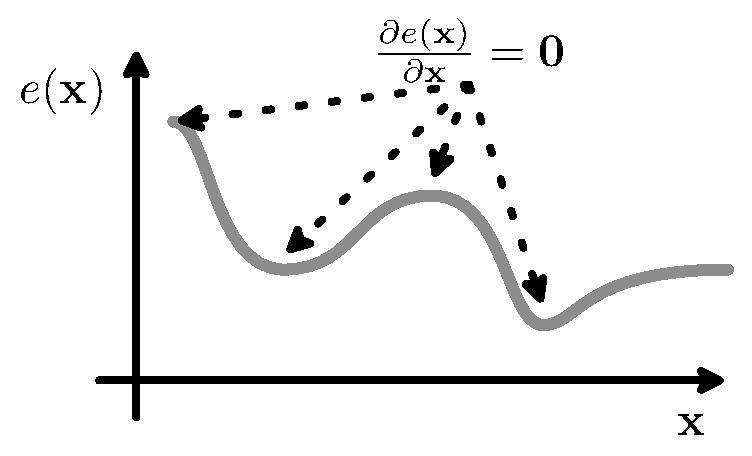
\includegraphics[width=0.8\textwidth]{chapters/minimization-fx/minimoex2.eps}
         \caption{$\VECTOR{b} \neq \VECTOR{f}(\VECTOR{x})$.}
         \label{fig:ex0b}
     \end{subfigure}
     \hfill
     \begin{subfigure}[b]{0.48\textwidth}
         \centering
         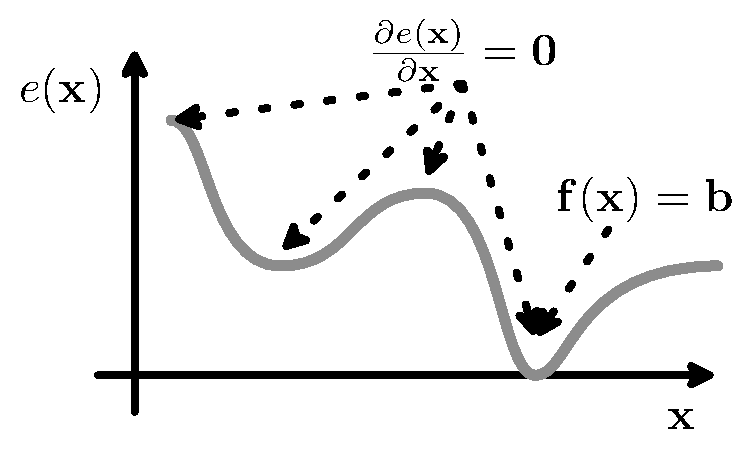
\includegraphics[width=0.8\textwidth]{chapters/minimization-fx/minimoex1.eps}
         \caption{$\VECTOR{b} = \VECTOR{f}(\VECTOR{x})$.}
         \label{fig:ex0a}
     \end{subfigure}
        \caption{Possibilidades para $\frac{\partial e(\VECTOR{x})}{\partial \VECTOR{x} }$.}
        \label{fig:ex0}
\end{figure}


Por outro lado, podemos realizar uma aproximação linear de $\VECTOR{f}(\VECTOR{x})$ em $e(\VECTOR{x})$
ao redor do ponto $\VECTOR{p}$ usando a \hyperref[def:taylor]{\textbf{série de Taylor}},
de modo que a Eq. (\ref{eq:proof:minfxbCfxb0}) pode ficar expresada como
\begin{equation}\label{eq:proof:minfxbCfxb0approx}
e(\VECTOR{x}) \approx ||\MATRIX{J}(\VECTOR{p})(\VECTOR{x}-\VECTOR{p})-(\VECTOR{b}-\VECTOR{f}(\VECTOR{p}))||_{\MATRIX{C}}^2,
\end{equation}
onde $\MATRIX{J}(\VECTOR{p})$ representa a \hyperref[def:jacobian]{\textbf{matriz Jacobiana}} 
de $\VECTOR{f}(\VECTOR{x})$ avaliada no ponto $\VECTOR{p}$.
Assim, usando o resultado da Prova \ref{proof:theo:minAxbCAxb} na Eq. (\ref{eq:proof:minfxbCfxb0approx}), 
podemos concluir que um ponto $\VECTOR{x}^*$ que é 
um mínimo da aproximação linear feita em $e(\VECTOR{x})$ ao redor do ponto $\VECTOR{p}$,
pode ser achado como
\begin{equation}\label{eq:proof:minAxbCAxb2approx}
\VECTOR{x}^* \approx \VECTOR{p}+ \left[ \MATRIX{J}(\VECTOR{p})^{\transpose}\MATRIX{C}\MATRIX{J}(\VECTOR{p}) \right]^{-1} \MATRIX{J}(\VECTOR{p})^{\transpose}\MATRIX{C} \left[\VECTOR{b}-\VECTOR{f}(\VECTOR{p})\right].
\end{equation}


Desta equação podemos tirar a seguintes conclusões:
\begin{itemize}

\item Observamos que a posição $\VECTOR{p}$ é corregida para ficar próximo à posição $\VECTOR{x}^*$, 
que é o valor mínimo na aproximação linear ao redor de $\VECTOR{p}$;
pelo que se deduz que a Eq. (\ref{eq:proof:minAxbCAxb2approx})
pode ser usada para procurar aproximações de pontos mínimos $\VECTOR{\hat{x}}$ em $e(\VECTOR{x})$ desde a posição $\VECTOR{p}$,
ou pelo menos aproximações de novas posições em caminhos numa direção descendente de $e(\VECTOR{x})$.

\item A Eq. (\ref{eq:proof:minAxbCAxb2approx}) é satisfeita 
com $\VECTOR{x}^* \approx \VECTOR{p}$ se acharmos um  
ponto $\VECTOR{p}$ onde  $\VECTOR{b} \approx \VECTOR{f}(\VECTOR{p})$; 
é dizer um mínimo global de $e(\VECTOR{x})$ em $\VECTOR{p}$, como pode ser visto na Figura \ref{fig:ex0a}. 

\item Se reescrevemos a Eq. (\ref{eq:proof:minAxbCAxb2approx}) usando o Teorema \ref{theo:derfxbCfxb0},
obtemos
\begin{equation}\label{eq:proof:minfxbCfxb2ea}
\VECTOR{x}^* \approx \VECTOR{p} -
0.5 \left[ \MATRIX{J}(\VECTOR{p})^{\transpose}\MATRIX{C} \MATRIX{J}(\VECTOR{p}) \right]^{-1}
\frac{\partial e(\VECTOR{p})}{\partial \VECTOR{x} },
\end{equation}
onde a Eq. (\ref{eq:proof:minfxbCfxb2ea}) é satisfeita 
com $\VECTOR{x}^* \approx \VECTOR{p}$
se acharmos um  ponto $\VECTOR{p}$ onde  
$\frac{\partial e(\VECTOR{p})}{\partial \VECTOR{x} }\approx \VECTOR{0}$; 
é dizer $\VECTOR{p}$ é um ponto de inflexão de $e(\VECTOR{x})$, como pode ser visto na Figura \ref{fig:ex0b}.
Porém, dado que a equação avança desde $\VECTOR{p}$ na direção de um mínimo $\VECTOR{x}^*$, 
mesmo que nos pontos de inflexão correspondentes a máximos ou pontos de sela,
encontremos valores de $\VECTOR{p}$ próximos a $\VECTOR{x}^*$,
 estes casos serão pouco estáveis pois
a correção da posição $\VECTOR{p}$ será na direção de um mínimo e não do máximo,
pois seguindo o Teorema \ref{theo:semipositivematrix1} a 
matriz $\MATRIX{J}(\VECTOR{p})^{\transpose}\MATRIX{C} \MATRIX{J}(\VECTOR{p})$ é 
semidefinida positiva se $\MATRIX{C}$ é simétrica.

\item Se modificamos a Eq. (\ref{eq:proof:minAxbCAxb2approx}), e escolhemos um ponto  
$\VECTOR{p}_0$ que consideremos próximo ao ponto $\VECTOR{\hat{x}}$ que minimiza $e(\VECTOR{\hat{x}})$,
podemos achar iterativamente aproximações lineares $\VECTOR{x}^*$ cada vez mais próximos a  $\VECTOR{\hat{x}}$,
se usamos a seguinte equação iterativa,
\begin{equation}\label{eq:proof:minfxbCfxb3}
\VECTOR{p}_{k} \leftarrow \VECTOR{p}_{k-1} -
\left[ \MATRIX{J}(\VECTOR{p}_{k-1})^{\transpose}\MATRIX{C} \MATRIX{J}(\VECTOR{p}_{k-1}) \right]^{-1}
\MATRIX{J}(\VECTOR{p}_{k-1})^{\transpose}\MATRIX{C} \left(\VECTOR{f}(\VECTOR{p}_{k-1})-\VECTOR{b}\right),
\end{equation}
iniciando desde um $\VECTOR{p}_{0}$, 
ate que exista uma tendência prolongada onde se observe que $\VECTOR{p}_{k}$ é muito próximo a $\VECTOR{p}_{k-1}$,
momento no qual declaramos que $\VECTOR{\hat{x}} \approx \VECTOR{p}_{k}$.
\item Como foi visto na Figura  \ref{fig:ex0b},
pode existir um mínimo global $\VECTOR{\hat{x}}$ de $e(\VECTOR{\hat{x}})>0$.
Isto nos restringe a que no uso da Eq. (\ref{eq:proof:minfxbCfxb3}),
nosso critério principal para estabelecer o final do cáculo iterativo,
deve ser a tendência na  proximidade entre $\VECTOR{p}_{k}$ e $\VECTOR{p}_{k-1}$ 
e não o valor de $e(\VECTOR{x}_k)$.
\end{itemize}~

Um diagrama completo resumindo todas estas conclusões pode ser visto na Figura \ref{fig:fluxo1}.
\end{myproofT}
\begin{figure}[!h]
     \centering
         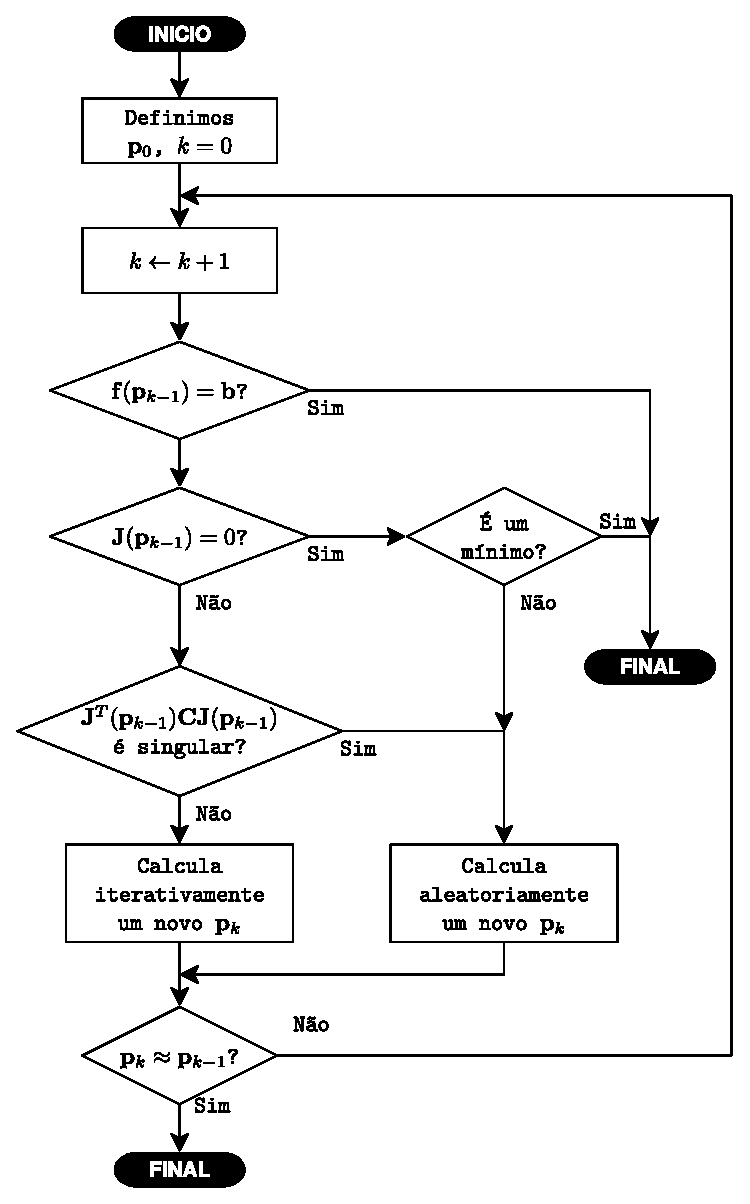
\includegraphics[width=0.75\textwidth]{chapters/minimization-fx/fluxo1.eps}
        \caption{Diagrama de fluxo da solução iterativa para achar um mínimo, seguindo a Prova \ref{proof:theo:minfxbCfxb}.}
        \label{fig:fluxo1}
\end{figure}


%%%%%%%%%%%%%%%%%%%%%%%%%%%%%%%%%%%%%%%%%%%%%%%%%%%%%%%%%%%%%%%%%%%%%%%%%%%%%%%%%%%%%%%
%%%%%%%%%%%%%%%%%%%%%%%%%%%%%%%%%%%%%%%%%%%%%%%%%%%%%%%%%%%%%%%%%%%%%%%%%%%%%%%%%%%%%%%
\begin{myproofT}[Relativa ao Teorema \ref{theo:minfxbCfxbaxqaxq}]\label{proof:theo:minfxbCfxbaxqd}
Dados,
um escalar $\alpha\in \mathbb{R}_+$,
os vetores coluna $\VECTOR{x}\in \mathbb{R}^N$, 
$\VECTOR{q}\in \mathbb{R}^N$ e
$\VECTOR{b}\in \mathbb{R}^M$,  
uma função $\VECTOR{f}:\mathbb{R}^{N} \rightarrow \mathbb{R}^{M}$, 
as matrizes diagonais $\MATRIX{C} \in \mathbb{R}^{M\times M}_+$ e $\MATRIX{D} \in \mathbb{R}^{N\times N}_+$, e 
definida a Eq. (\ref{eq:proof:minfxbCfxbaxqd0}),
\begin{equation}\label{eq:proof:minfxbCfxbaxqd0}
e(\VECTOR{x})=||\VECTOR{f}(\VECTOR{x})-\VECTOR{b}||_{\MATRIX{C}}^2+\alpha||\VECTOR{x}-\VECTOR{q}||_{\MATRIX{D}}^2;
\end{equation}
sabemos que para achar o ponto $\VECTOR{x}=\VECTOR{\hat{x}}$ que gere o menor valor de $e(\VECTOR{x})$, é aplicado
o critério que um ponto de inflexão $\VECTOR{x}^+$; é dizer, um máximo, um mínimo ou um ponto de sela, pode ser achado quando 
$\frac{\partial e(\VECTOR{x}^+)}{\partial \VECTOR{x} }=[0~ 0~ \hdots~ 0 ]^{\transpose}$ (ver Figura \ref{fig:ex0b});
assim, usando o Teorema \ref{theo:derfxbCfxb0} e o Corolário \ref{coro:derAxbAxb2} obtemos que
\begin{equation}\label{eq:proof:minfxbCfxb1exact2}
2 \MATRIX{J}(\VECTOR{x}^+)^{\transpose}\MATRIX{C}\left[ \VECTOR{f}(\VECTOR{x}^+)-\VECTOR{b} \right] +
2 \alpha\MATRIX{D}\left[\VECTOR{x}^+-\VECTOR{q}\right]
=
\frac{\partial e(\VECTOR{x}^+)}{\partial \VECTOR{x} }=[0~ 0~ \hdots~ 0 ]^{\transpose},
\end{equation}
Da Eq. (\ref{eq:proof:minfxbCfxb1exact2}) observamos, 
que podemos achar um ponto de inflexão $\VECTOR{q}$
em $e(\VECTOR{q})$ se 
$\MATRIX{J}(\VECTOR{q})  = \MATRIX{0}$ ou um mínimo geral se $\VECTOR{f}(\VECTOR{q})=\VECTOR{b}$,
caso contrario, 
se nenhuma destas possibilidades são cumpridas devemos aplicar outros critérios para achar os pontos de inflexão.

Assim, procurando outros critérios, podemos realizar uma aproximação linear de $\VECTOR{f}(\VECTOR{x})$ em $e(\VECTOR{x})$
ao redor do ponto $\VECTOR{p}$ usando a \hyperref[def:taylor]{\textbf{série de Taylor}},
de modo que a Eq. (\ref{eq:proof:minfxbCfxbaxqd0}) pode ficar expressada como
\begin{equation}\label{eq:proof:minfxbCfxb0alphaxqDapprox}
e(\VECTOR{x}) \approx 
||\MATRIX{J}(\VECTOR{p})[\VECTOR{x}-\VECTOR{p}]-[\VECTOR{b}-\VECTOR{f}(\VECTOR{p})]||_{\MATRIX{C}}^2+
\alpha||[\VECTOR{x}-\VECTOR{p}]-[\VECTOR{q}-\VECTOR{p}]||_{\MATRIX{D}}^2,
\end{equation}
onde $\MATRIX{J}(\VECTOR{p})$ representa a \hyperref[def:jacobian]{\textbf{matriz Jacobiana}} 
de $\VECTOR{f}(\VECTOR{x})$ avaliada no ponto $\VECTOR{p}$.
Assim, usando o resultado da Prova \ref{proof:theo:minAxbCAxbalphaxqD} na Eq. (\ref{eq:proof:minfxbCfxb0alphaxqDapprox}), 
podemos concluir que um ponto $\VECTOR{x}^*$ que é 
um mínimo da aproximação linear feita em $e(\VECTOR{x})$ ao redor do ponto $\VECTOR{p}$,
pode ser achado como
\begin{equation}\label{eq:proof:minfxbCfxbaxqd2}
\VECTOR{x}^* \approx \VECTOR{p} +
\left[ \MATRIX{J}(\VECTOR{p})^{\transpose}\MATRIX{C} \MATRIX{J}(\VECTOR{p})+\alpha \MATRIX{D} \right]^{-1}
\left\{ \MATRIX{J}(\VECTOR{p})^{\transpose}\MATRIX{C} \left[\VECTOR{b}-\VECTOR{f}(\VECTOR{p})\right]-\alpha\MATRIX{D}[\VECTOR{p}-\VECTOR{q}]\right\}.
\end{equation}


Desta equação podemos tirar a seguintes conclusões:
\begin{itemize}

\item Observamos que a posição $\VECTOR{p}$ é corregida para ficar próximo à posição $\VECTOR{x}^*$, 
que é o valor mínimo na aproximação linear ao redor de $\VECTOR{p}$;
pelo que se deduz que a Eq. (\ref{eq:proof:minfxbCfxbaxqd2})
pode ser usada para procurar aproximações de pontos mínimos $\VECTOR{\hat{x}}$ em $e(\VECTOR{x})$ desde a posição $\VECTOR{p}$,
ou pelo menos aproximações de novas posições em caminhos numa direção descendente 
de $e(\VECTOR{x})$ desde a posição $\VECTOR{p}$.

\begin{comment}
\item A Eq. (\ref{eq:proof:minfxbCfxbaxqd2}) é satisfeita 
com $\VECTOR{x}^* \approx \VECTOR{p}$ se acharmos um  
ponto $\VECTOR{p}$ onde  $\VECTOR{b} \approx \VECTOR{f}(\VECTOR{p}\approx \VECTOR{q})$; 
é dizer um mínimo global de $e(\VECTOR{x})$ em $\VECTOR{p}$, como pode ser visto na Figura \ref{fig:ex0a}. 
\end{comment}

\item Se reescrevemos a Eq. (\ref{eq:proof:minfxbCfxbaxqd2}) usando o Teorema \ref{theo:derfxbCfxb0}
e o Corolário \ref{coro:derAxbAxb2},
obtemos
\begin{equation}\label{eq:proof:minfxbCfxb2ea1}
\VECTOR{x}^* \approx \VECTOR{p} -
0.5 \left[ \MATRIX{J}(\VECTOR{p})^{\transpose}\MATRIX{C} \MATRIX{J}(\VECTOR{p})+\alpha \MATRIX{D} \right]^{-1}
\frac{\partial e(\VECTOR{p})}{\partial \VECTOR{x} },
\end{equation}
onde a Eq. (\ref{eq:proof:minfxbCfxb2ea1}) é satisfeita 
com $\VECTOR{x}^* \approx \VECTOR{p}$
se acharmos um  ponto $\VECTOR{p}$ onde  
$\frac{\partial e(\VECTOR{p})}{\partial \VECTOR{x} }\approx \VECTOR{0}$,
 como descrito na Eq. (\ref{eq:proof:minfxbCfxb1exact2}); 
é dizer $\VECTOR{p}$ é um ponto de inflexão de $e(\VECTOR{x})$, ver Figura \ref{fig:ex0b}.
Porém, dado que a equação avança desde $\VECTOR{p}$ na direção de um mínimo $\VECTOR{x}^*$, 
mesmo que nos pontos de inflexão correspondentes a máximos ou pontos de sela,
encontremos valores de $\VECTOR{p}$ próximos a $\VECTOR{x}^*$,
 estes casos serão pouco estáveis pois
a correção da posição $\VECTOR{p}$ será na direção de um mínimo e não do máximo.

\item Se modificamos a Eq. (\ref{eq:proof:minfxbCfxbaxqd2}), e escolhemos um ponto  
$\VECTOR{p}_0$ que consideremos próximo ao ponto $\VECTOR{x}=\VECTOR{\hat{x}}$ que minimiza $e(\VECTOR{x})$,
podemos achar iterativamente aproximações lineares $\VECTOR{x}^*$ cada vez mais próximos a  $\VECTOR{\hat{x}}$,
se usamos a seguinte equação iterativa,
\begin{equation}\label{eq:proof:minfxbCfxb3a}
\VECTOR{p}_{k} \leftarrow \VECTOR{p}_{k-1} -
\left[ \MATRIX{J}(\VECTOR{p}_{k-1})^{\transpose}\MATRIX{C} \MATRIX{J}(\VECTOR{p}_{k-1}) +\alpha \MATRIX{D}\right]^{-1}
\left\{ \MATRIX{J}(\VECTOR{p}_{k-1})^{\transpose}\MATRIX{C} \left[\VECTOR{f}(\VECTOR{p}_{k-1})-\VECTOR{b}\right]+
\alpha\MATRIX{D}[\VECTOR{p}_{k-1}-\VECTOR{q}]\right\},
\end{equation}
iniciando desde um $\VECTOR{p}_{0}$ 
ate que exista uma tendência prolongada onde se observe que $\VECTOR{p}_{k}$ é muito próximo a $\VECTOR{p}_{k-1}$,
momento no qual declaramos que $\VECTOR{\hat{x}} \approx \VECTOR{p}_{k}$.
\item Como foi visto na Figura  \ref{fig:ex0b},
pode existir um mínimo global $\VECTOR{x}=\VECTOR{\hat{x}}$ de $e(\VECTOR{x}) > 0$.
Isto nos restringe a que no uso da Eq. (\ref{eq:proof:minfxbCfxb3a}),
nosso critério principal para estabelecer o final do cáculo iterativo,
deve ser a tendência na  proximidade entre $\VECTOR{p}_{k}$ e $\VECTOR{p}_{k-1}$ 
e não o valor de $e(\VECTOR{x}_k)$.
\end{itemize}

Um diagrama completo resumindo todas estas conclusões pode ser visto na Figura \ref{fig:fluxo2}.
\end{myproofT}
\begin{figure}[!h]
     \centering
         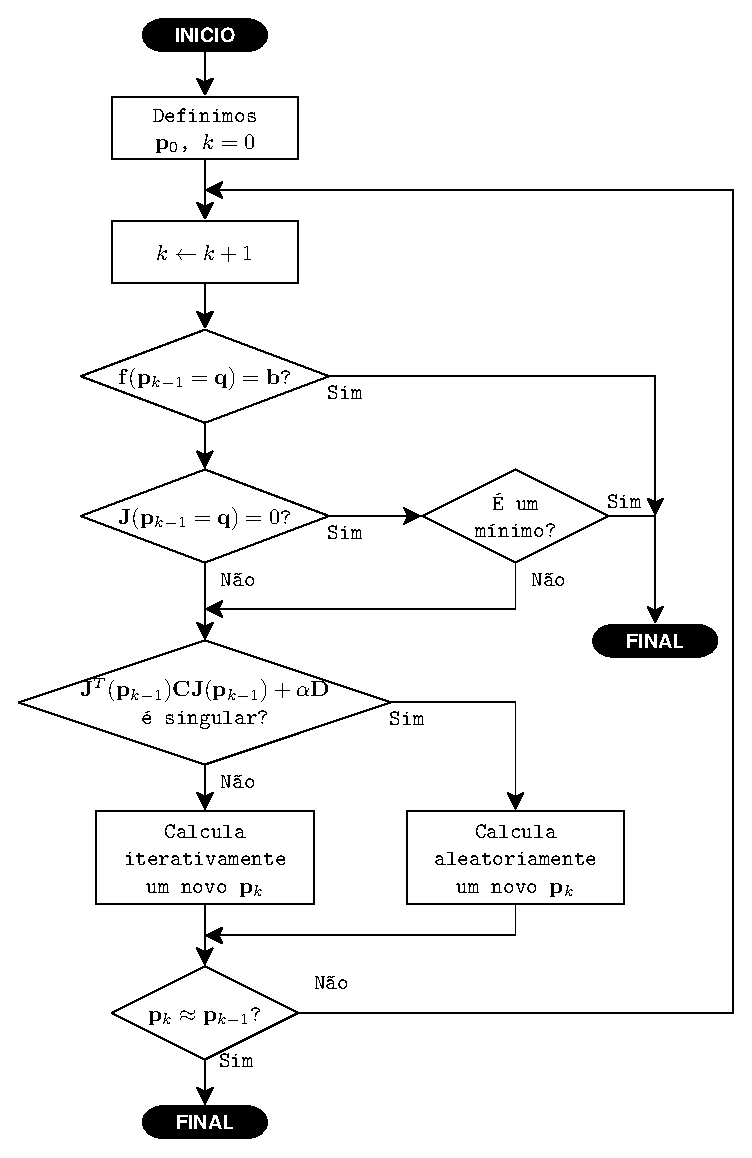
\includegraphics[width=0.75\textwidth]{chapters/minimization-fx/fluxo2.eps}
        \caption{Diagrama de fluxo da solução iterativa para achar um mínimo, seguindo a Prova \ref{proof:theo:minfxbCfxbaxqd}.}
        \label{fig:fluxo2}
\end{figure}

%%%%%%%%%%%%%%%%%%%%%%%%%%%%%%%%%%%%%%%%%%%%%%%%%%%%%%%%%%%%%%%%%%%%%%%%%%%%%%%%%%%%%%%
%%%%%%%%%%%%%%%%%%%%%%%%%%%%%%%%%%%%%%%%%%%%%%%%%%%%%%%%%%%%%%%%%%%%%%%%%%%%%%%%%%%%%%%
\begin{myproofT}[Relativa ao Teorema \ref{theo:minfxbCfxbaxoaxo}]\label{proof:theo:minfxbCfxbaxod}
Dados,
um escalar $\alpha\in \mathbb{R}_+$,
os vetores coluna $\VECTOR{x}\in \mathbb{R}^N$, 
$\VECTOR{x}_{last}\in \mathbb{R}^N$ e
$\VECTOR{b}\in \mathbb{R}^M$,  
uma função $\VECTOR{f}:\mathbb{R}^{N} \rightarrow \mathbb{R}^{M}$, 
as matrizes diagonais $\MATRIX{C} \in \mathbb{R}^{M\times M}$ e $\MATRIX{D} \in \mathbb{R}^{N\times N}$, e 
definida a Eq. (\ref{eq:proof:minfxbCfxbaxod0}),
\begin{equation}\label{eq:proof:minfxbCfxbaxod0}
e(\VECTOR{x})=||\VECTOR{f}(\VECTOR{x})-\VECTOR{b}||_{\MATRIX{C}}^2+\alpha||\VECTOR{x}-\VECTOR{x}_{last}||_{\MATRIX{D}}^2,
\end{equation}
tendo em consideração que $\VECTOR{x}_{last}$ é uma constante equivalente a $\VECTOR{x}_{k-1}$
numa busca iterativa ou equivalente a $\VECTOR{p}$, 
se decidimos usar uma aproximação linear ao redor de $\VECTOR{p}$ em $\VECTOR{f}(\VECTOR{x})$; 
é dizer, o segundo somando na Eq. (\ref{eq:proof:minfxbCfxbaxod0}) 
procura minimizar $||\VECTOR{x}_{k}-\VECTOR{x}_{k-1}||_{\MATRIX{D}}^2$.

Sabemos que para achar o ponto $\VECTOR{x}=\VECTOR{\hat{x}}$ que gere o menor valor de $e(\VECTOR{x})$, é aplicado
o critério que um ponto de inflexão $\VECTOR{x}^+$; é dizer, um máximo, um mínimo ou um ponto de sela, pode ser achado quando 
$\frac{\partial e(\VECTOR{x}^+)}{\partial \VECTOR{x} }=[0~ 0~ \hdots~ 0 ]^{\transpose}$ (ver Figura \ref{fig:ex0b});
assim, usando o Teorema \ref{theo:derfxbCfxb0} e o Corolário \ref{coro:derAxbAxb2} obtemos que
\begin{equation}\label{eq:proof:minfxbCfxbaxod1exact2}
2 \MATRIX{J}(\VECTOR{x}^+)^{\transpose}\MATRIX{C}\left[ \VECTOR{f}(\VECTOR{x}^+)-\VECTOR{b} \right] +
2 \alpha\MATRIX{D}\left[\VECTOR{x}^+-\VECTOR{x}_{last}\right]
=
\frac{\partial e(\VECTOR{x}^+)}{\partial \VECTOR{x} }=[0~ 0~ \hdots~ 0 ]^{\transpose}.
\end{equation}
Da Eq. (\ref{eq:proof:minfxbCfxbaxod1exact2}) observamos, 
que podemos achar um ponto de inflexão $\VECTOR{x}^+=\VECTOR{x}_{last}$
em $e(\VECTOR{x}_{last})$ se 
$\MATRIX{J}(\VECTOR{x}_{last})  = \MATRIX{0}$ ou um mínimo geral se $\VECTOR{f}(\VECTOR{x}_{last})=\VECTOR{b}$,
caso contrario, 
se nenhuma destas possibilidades são cumpridas devemos aplicar outros critérios para achar os pontos de inflexão.



Assim, procurando outros critérios, podemos igualar $\VECTOR{x}_{last}\equiv \VECTOR{p}$ e 
realizar uma aproximação linear de $\VECTOR{f}(\VECTOR{x})$ em $e(\VECTOR{x})$
ao redor do ponto $\VECTOR{p}$ usando a \hyperref[def:taylor]{\textbf{série de Taylor}} truncada,
de modo que a Eq. (\ref{eq:proof:minfxbCfxbaxod0}) pode ficar expressada como
\begin{equation}\label{eq:proof:minfxbCfxbaxod0alphaxqDapprox}
e(\VECTOR{x}) \approx e_{\VECTOR{p}}(\VECTOR{x})  \equiv 
||\MATRIX{J}(\VECTOR{p})[\VECTOR{x}-\VECTOR{p}]-[\VECTOR{b}-\VECTOR{f}(\VECTOR{p})]||_{\MATRIX{C}}^2+
\alpha||\VECTOR{x}-\VECTOR{p}||_{\MATRIX{D}}^2,
\end{equation}
onde $\MATRIX{J}(\VECTOR{p})$ representa a \hyperref[def:jacobian]{\textbf{matriz Jacobiana}} 
de $\VECTOR{f}(\VECTOR{x})$ avaliada no ponto $\VECTOR{p}$.
Assim, usando o resultado da Prova \ref{proof:theo:minAxbCAxbalphaxqD} na Eq. (\ref{eq:proof:minfxbCfxbaxod0alphaxqDapprox}), 
onde se aplica que $\frac{\partial e_{\VECTOR{p}}(\VECTOR{x}^*)}{\partial \VECTOR{x} }=\VECTOR{0}$,
podemos concluir que um ponto $\VECTOR{x}^*$ que é 
um mínimo da aproximação linear feita em $e(\VECTOR{x})$ ao redor do ponto $\VECTOR{p}$,
pode ser achado como,
\begin{equation}\label{eq:proof:minfxbCfxbaxod2}
\VECTOR{x}^* \approx \VECTOR{p} +
\left[ \MATRIX{J}(\VECTOR{p})^{\transpose}\MATRIX{C} \MATRIX{J}(\VECTOR{p})+\alpha \MATRIX{D} \right]^{-1}
\MATRIX{J}(\VECTOR{p})^{\transpose}\MATRIX{C} \left[\VECTOR{b}-\VECTOR{f}(\VECTOR{p})\right].
\end{equation}

Desta equação podemos tirar a seguintes conclusões:
\begin{itemize}

\item Observamos que a posição $\VECTOR{p}$ é corregida para ficar próximo à posição $\VECTOR{x}^*$, 
que é o valor mínimo na aproximação linear ao redor de $\VECTOR{p}$;
pelo que se deduz que a Eq. (\ref{eq:proof:minfxbCfxbaxod2})
pode ser usada para procurar aproximações de pontos mínimos $\VECTOR{\hat{x}}$ em $e(\VECTOR{x})$ desde a posição $\VECTOR{p}$,
ou pelo menos aproximações de novas posições em caminhos numa direção descendente de $e(\VECTOR{x})$.

\item A Eq. (\ref{eq:proof:minfxbCfxbaxod2}) é satisfeita 
com $\VECTOR{x}^* \approx \VECTOR{p}$ se acharmos um  
ponto $\VECTOR{p}$ onde  $\VECTOR{b} \approx \VECTOR{f}(\VECTOR{p}\approx \VECTOR{x}_{last})$; 
é dizer um mínimo global de $e(\VECTOR{x})$ em $\VECTOR{p}$, como pode ser visto na Figura \ref{fig:ex0a}. 

\item Se reescrevemos a Eq. (\ref{eq:proof:minfxbCfxbaxod2}) usando o Teorema \ref{theo:derfxbCfxb0}
e o Corolário \ref{coro:derAxbAxb2},
obtemos
\begin{equation}\label{eq:proof:minfxbCfxbaxod2ea1}
\VECTOR{x}^* \approx \VECTOR{p} -
0.5 \left[ \MATRIX{J}(\VECTOR{p})^{\transpose}\MATRIX{C} \MATRIX{J}(\VECTOR{p})+\alpha \MATRIX{D} \right]^{-1}
\frac{\partial e(\VECTOR{p})}{\partial \VECTOR{x} },
\end{equation}
onde a Eq. (\ref{eq:proof:minfxbCfxbaxod2ea1}) é satisfeita 
com $\VECTOR{x}^* \approx \VECTOR{p}$
se acharmos um  ponto $\VECTOR{p}$ onde  
$\frac{\partial e(\VECTOR{p})}{\partial \VECTOR{x} }\approx \VECTOR{0}$; 
é dizer $\VECTOR{p}$ é um ponto de inflexão de $e(\VECTOR{x})$, como pode ser visto na Figura \ref{fig:ex0b}.
Porém, dado que a equação avança desde $\VECTOR{p}$ na direção de um mínimo $\VECTOR{x}^*$, 
mesmo que nos pontos de inflexão correspondentes a máximos ou pontos de sela,
encontremos valores de $\VECTOR{p}$ próximos a $\VECTOR{x}^*$,
 estes casos serão pouco estáveis pois
a correção da posição $\VECTOR{p}$ será na direção de um mínimo e não do máximo.
\item Seguindo o Teorema \ref{theo:semipositivematrix1}, se $\MATRIX{C}$ e $\MATRIX{D}$ são simétricas, 
então a matriz $\MATRIX{J}(\VECTOR{p})^{\transpose}\MATRIX{C} \MATRIX{J}(\VECTOR{p})+\alpha \MATRIX{D}$
é semidefinida positiva.

\item Se modificamos a Eq. (\ref{eq:proof:minfxbCfxbaxod2}), e escolhemos um ponto  
$\VECTOR{p}_0$ que consideremos próximo ao ponto $\VECTOR{x}=\VECTOR{\hat{x}}$ que minimiza $e(\VECTOR{x})$,
podemos achar iterativamente aproximações lineares $\VECTOR{x}^*$ cada vez mais próximos a  $\VECTOR{\hat{x}}$,
se usamos a seguinte equação iterativa,
\begin{equation}\label{eq:proof:minfxbCfxbaxod3b}
\VECTOR{p}_{k} \leftarrow \VECTOR{p}_{k-1} -
\left[ \MATRIX{J}(\VECTOR{p}_{k-1})^{\transpose}\MATRIX{C} \MATRIX{J}(\VECTOR{p}_{k-1}) +\alpha \MATRIX{D}\right]^{-1}
\MATRIX{J}(\VECTOR{p}_{k-1})^{\transpose}\MATRIX{C} \left[\VECTOR{f}(\VECTOR{p}_{k-1})-\VECTOR{b}\right],
\end{equation}
onde se inicia desde um $\VECTOR{p}_{0}$ 
ate que exista uma tendência prolongada onde se observe que $\VECTOR{p}_{k}$ é muito próximo a $\VECTOR{p}_{k-1}$,
momento no qual declaramos que $\VECTOR{\hat{x}} \approx \VECTOR{p}_{k}$.
Disto também se deduz que o erro a minimizar em cada iteração será diferente e influenciado pelo valor do ponto $\VECTOR{p}_{k-1}$,
\begin{equation}
e_{k-1}(\VECTOR{x})  \equiv 
||\VECTOR{f}(\VECTOR{x})-\VECTOR{b}||_{\MATRIX{C}}^2+
\alpha||\VECTOR{x}-\VECTOR{p}_{k-1}||_{\MATRIX{D}}^2
\end{equation}
\item Como foi visto na Figura  \ref{fig:ex0b},
pode existir um mínimo global $\VECTOR{x}=\VECTOR{\hat{x}}$ de $e(\VECTOR{x}) > 0$.
Isto nos restringe a que no uso da Eq. (\ref{eq:proof:minfxbCfxb3a}),
nosso critério principal para estabelecer o final do cálculo iterativo,
deve ser a tendência na  proximidade entre $\VECTOR{p}_{k}$ e $\VECTOR{p}_{k-1}$ 
e não o valor de $e(\VECTOR{x}_k)$.
\end{itemize}~

Um diagrama completo resumindo todas estas conclusões pode ser visto na Figura \ref{fig:fluxo3}.
\end{myproofT}
\begin{figure}[!h]
     \centering
         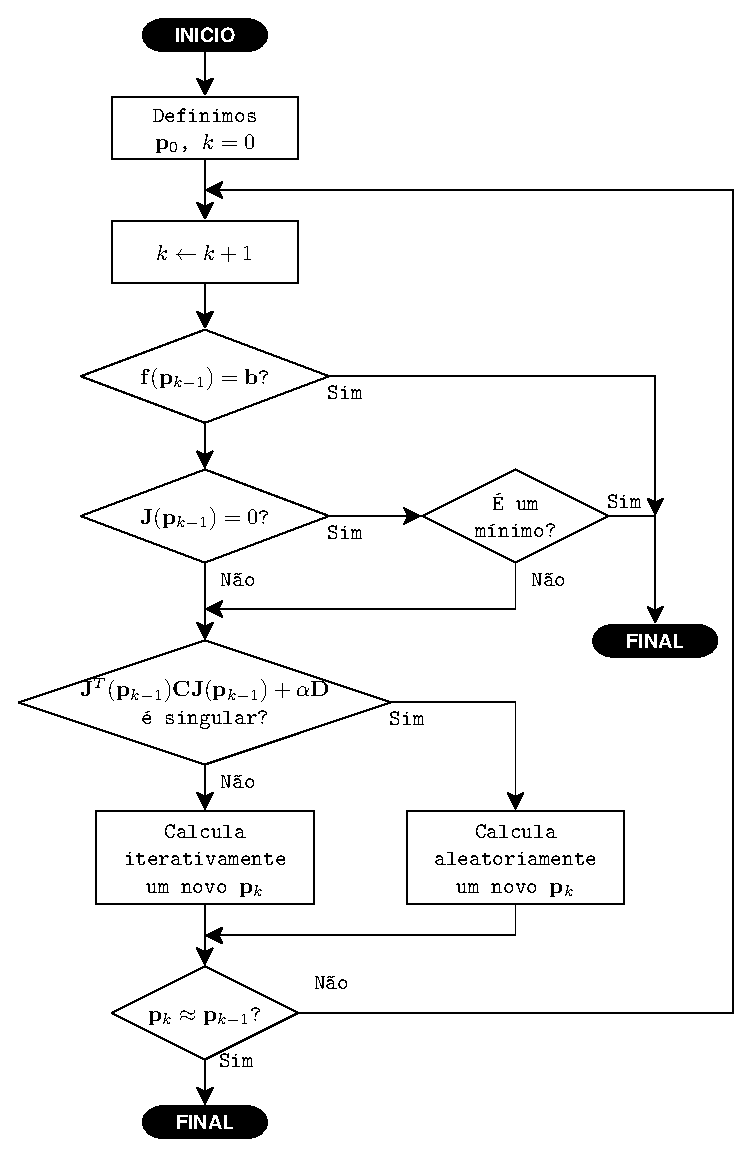
\includegraphics[width=0.75\textwidth]{chapters/minimization-fx/fluxo3.eps}
        \caption{Diagrama de fluxo da solução iterativa para achar um mínimo, seguindo a Prova \ref{proof:theo:minfxbCfxbaxod}.}
        \label{fig:fluxo3}
\end{figure}
